
\newcommand{\PaperTitleMapping}{Nonlinear grid mapping applied to an FDTD-based, multi-center 3D
                                  Schr\"odinger equation solver}

\section{\PaperTitleMapping}
\label{section:papers:qfdtd}

\begin{flushright}
Nicolas Bigaouette, Edward Ackad, Lora Ramunno\\
\textit{Computer Physics Communications} 183(1), 2012, 38–45\\
\href{http://dx.doi.org/10.1016/j.cpc.2011.08.011}{doi:10.1016/j.cpc.2011.08.011}
\end{flushright}

% Include PDF's abstract in the Table-of-Content as ``subsection 0'' but hide the number
\HidePDFAbstractNumber

\subsection{Author contributions}
The whole QFDTD package was written by N. B. The post processing and analysis
was performed entirely by N. B. The method developed to obtain eigenstates in
imaginary time is original work by N. B. The nonlinear mapping is original work
too but was inspired by conformal mapping as suggested by E. A. The whole text
was written by N. B. with inputs from L. R. and E. A. All authors contributed to
the discussion.

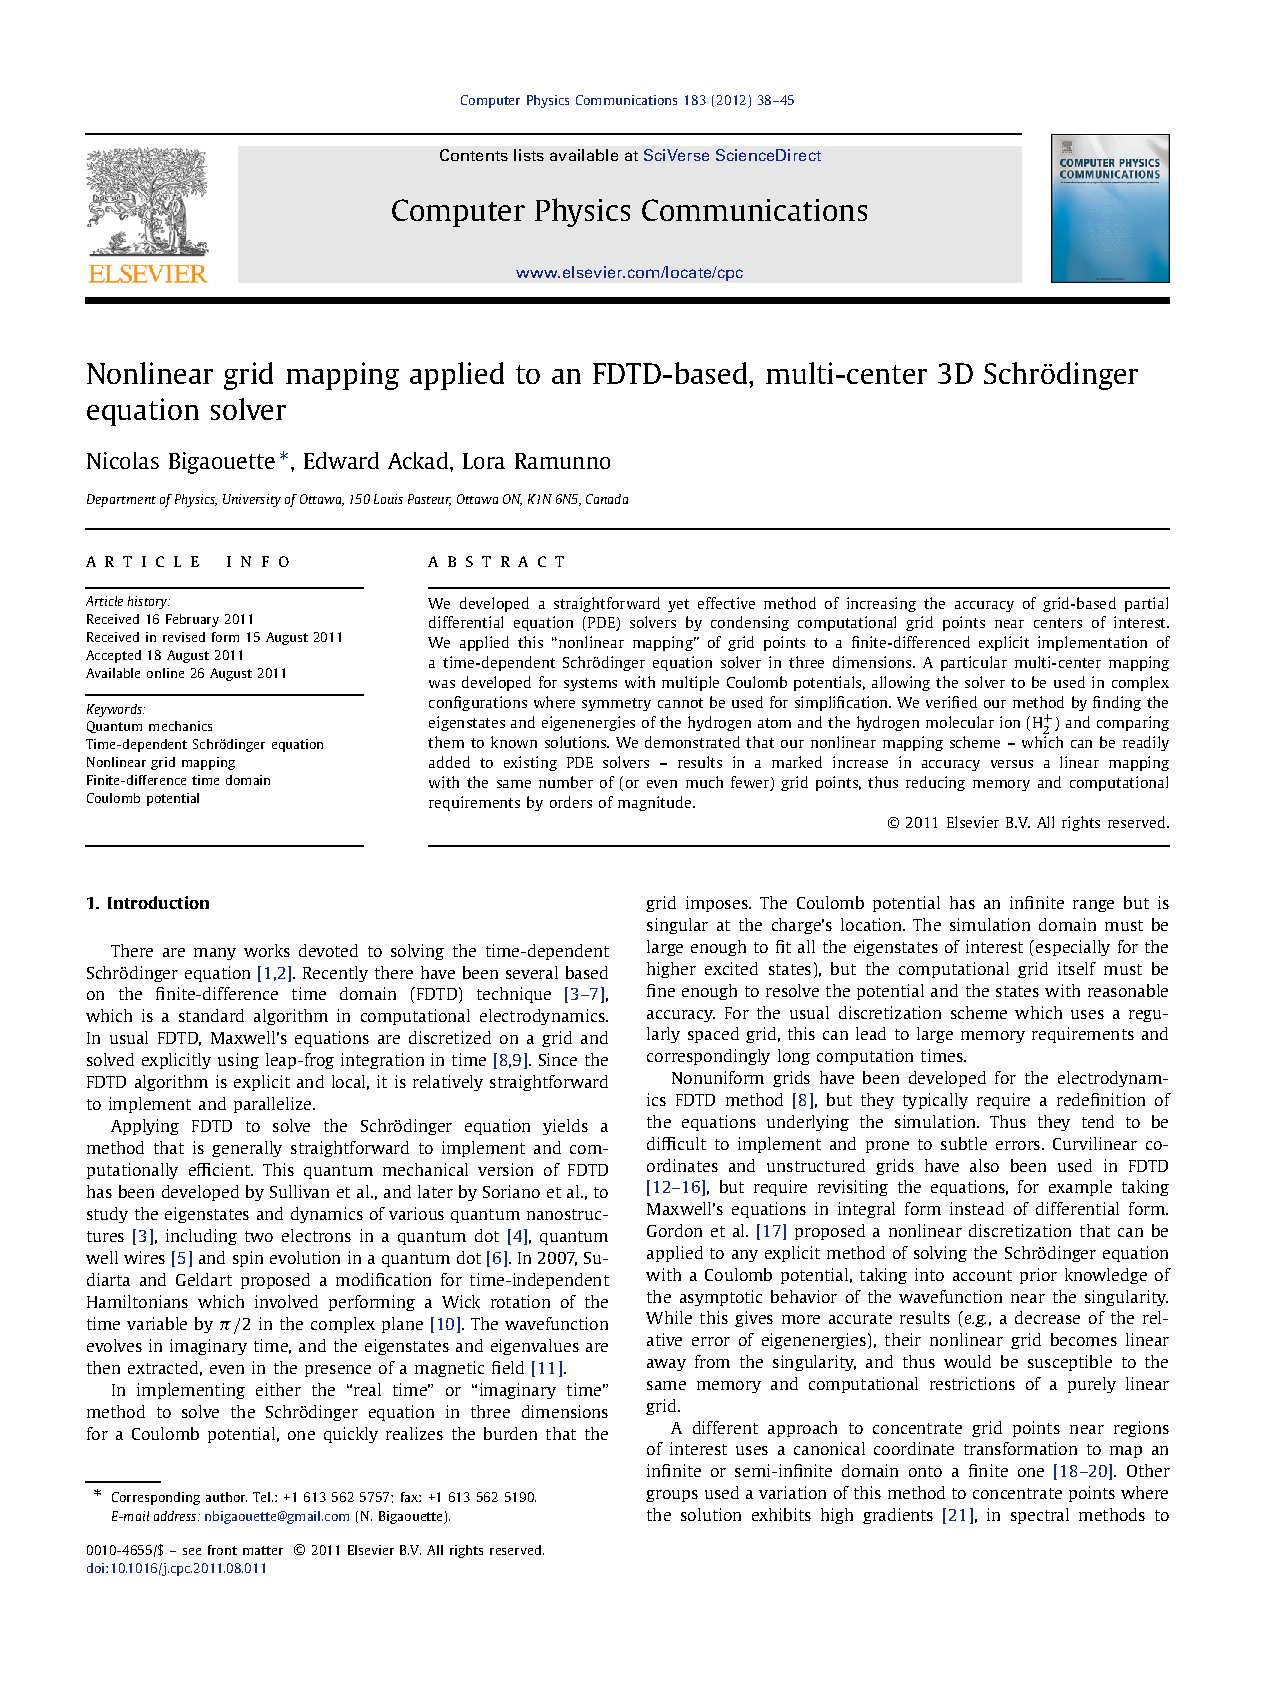
\includepdf[pages=-,
            addtotoc={
                %1,section,1,\PaperTitleMapping,paper_mapping,
                1,subsection,2,Abstract,paper_mapping_Abstract,
                1,subsection,2,Introduction,paper_mapping_intro,
                2,subsection,2,Finite-differenced Schrödinger equation,paper_mapping_fdtd,
                2,subsubsection,3,Real-time,paper_mapping_realtime,
                3,subsubsection,3,Imaginary-time,paper_mapping_imagtime,
                3,subsection,2,Details of nonlinear mapping,paper_mapping_details,
                4,subsubsection,3,General approach,paper_mapping_details_general,
                4,subsubsection,3,Details of the implementation,paper_mapping_details_details,
                5,subsubsection,3,Nonlinear mapping for the Coulomb potential,paper_mapping_details_coulomb,
                6,subsection,2,Validation and results,paper_mapping_results,
                6,subsubsection,3,Hydrogen atom,paper_mapping_results_h,
                7,subsubsection,3,Hydrogen cation molecule,paper_mapping_results_h2p,
                7,subsection,2,Conclusion,paper_mapping_conclusion,
                8,subsection,2,References,paper_mapping_ref
            }]{papers/Bigaouette2011_Mapping.pdf}
